%\todo[inline]{Rewrite so that it is not just the abstract restated.}
%Success in practice and heuristic arguments, like the above, have inspired a widespread belief that t-SNE visualizations preserve the cluster structure of the input. To the contrary, we prove that the strength of the input clustering cannot be reliably inferred from the low-dimensional visualization.



%Heuristic arguments, like the above, and success in practice and have inspired a widespread belief that the cluster structure present in t-SNE visualizations is in correspondence with the cluster structure of the input. 
%The practical success and appeal of t-SNE has inspired a b

%Suppose you have two datasets, and their t-SNE plots strongly suggest not only that the datasets are clustered but that they obey similar clusterings.

Previous works by \citet{linderman2019clustering} and \citet{arora2018analysis} have identified that clustered inputs induce clustered t-SNE visualizations in the sense that sufficiently well-separated Gaussian-shaped clusters in the input must produce corresponding well-separated clusters in the output visualization. %a suitable sense. 
A key question for practitioners left unanswered by these analyses is: when does a clustered output imply a clustered input? 
%Does a t-SNE output appear clustered if and only if the input is clustered? 
More generally, what information can be deduced about the input given a visualization? We begin to answer this question by proving that the strength of cluster separation in the input cannot be reliably inferred from the low-dimensional visualization. 
%In particular, we prove that (i) \textcolor{red}{identically clustered} %similarly clustered 
%t-SNE visualizations \textcolor{red}{may come from datasets with very different distance structure}%do not imply similarly clustered inputs
%, and (ii) \text{highly distinct} %ly clustered 
%visualizations \textcolor{red}{may come from datasets with very similar distance structure}.%do not imply distinctly different inputs. 

%similarly clustered outputs =/=> similarly strong clustering in input space.

%differently clustered outputs =/=> far apart inputs.


%Central to the widespread use of t-SNE and related methods is the conviction that they produce visualizations whose cluster structure roughly matches that of the input. To the contrary, we prove that the strength of the input clustering cannot be reliably inferred from the low-dimensional visualization.

%\todo[inline]{Add the definitions of the cluster indexes to appendix.}
To quantify the strength of cluster separation %the strength of the cluster \textcolor{red}{saliency} %structure 
in a dataset, we employ well-known distance-based cluster indices such as the average silhouette score \citep{rousseeuw1987silhouettes}, the Calinski-Harabasz index \citep{Caliński01011974}, and the Dunn index \citep{DunnIndex1974}. 
%At their core, these indices measure the cluster partition's salience by producing some ratio of inter-cluster and  intra-cluster distances. 
For sake of readability, we focus on presenting our results with respect to the average silhouette score. Our results hold identically for the other indices as well (see Appendices \ref{sec:CHindex} and \ref{sec:Dunnindex}). 

%, we focus on the Average Silhouette Score for the sake of presentation. The formal definitions and associated theorems of the other two indices can be found in Appendix \ref{sec:appendix_false_pos}. 

%\todo[inline]{Finish adding other two indices to appendix.}

%For an $n$-point dataset $\mathcal{X} = \{x_1, \dots, x_n\} \subset \mathbb{R}^{n-1}$ and a partition of the dataset into clusters $C_1 \sqcup C_2 \sqcup \dots \sqcup C_k = [n]$\footnote{In alignment with our usage of the cluster indexes and to avoid division by zero, we assume that for all $m \in [k], |C_m|>1$. {\color{red} Rewrite proof so this can be removed.}}, we denote the three indexes as $\bar{\mathcal{S}}(\mathcal{X}; C_{m\in[k]})$, -, and - for the Average Silhouette Score, the Calinski-Harabasz index, and the Davies-Bouldin index, respectively. You can see the range of each index in Table \ref{table:demo}.

\begin{definition}
    Given a partition $C_1 \sqcup C_2 \sqcup \dots \sqcup C_k = [n]$ of $n$ points $\{x_1,\ldots,x_n\} = X$ into $k \geq 2$ parts, the \textbf{silhouette score} of a point $x_i$, denoted \(\mathcal{S}(i)\), is the normalized difference between the average within- and the closest across-cluster distances from $x_i$: 
$$
\mathcal{S}(i) := \frac{b(i)-a(i)}{\max \{b(i),a(i)\}} 
\hspace{0.25in}
a(i) := \sum_{j \in C^{(i)}} \frac{\lVert x_i - x_j \rVert}{|C^{(i)}|-1} 
\hspace{0.25in}
b(i) := \min_{
\substack{m \in [k] \\ C_m \neq C^{(i)}}} \sum_{j \in C_m} \frac{\lVert x_i - x_j \rVert}{|C_m|},
$$
where $C^{(i)}$ is the cluster to which $i$ belongs. Note that if $|C^{(i)}|=1$, then $\mathcal{S}(i)$ is defined to be zero.
The \textbf{average silhouette score} then is simply the average across all points in $X$:
$$\bar{\mathcal{S}}(X; C_{m\in[k]}) := \frac{1}{n} \sum_{i \in [n]} \mathcal{S}(i).$$
\end{definition}
Observe that the (average) silhouette score ranges from $-1$ to $1$ with higher scores reflecting a large separation between clusters relative to cluster diameter. A score of zero reflects minimal separation between clusters, while negative values reflect cluster overlaps.

%a score of $1$ being assigned to maximally %clustered 
%\textcolor{red}{well-separated} data, $-1$ to \textcolor{red}{``incorrectly"} clustered data, and $0$ to unclustered data. %\textcolor{red}{inter-cluster distances}.

%%%%%%%%%%%%%%%%%%%%%%%
\iffalse
For an $n$-point dataset $X = \{x_1, \dots, x_n\} \subset \mathbb{R}^{n-1}$ and its partition into clusters $C_1 \sqcup C_2 \sqcup \dots \sqcup C_k = [n]$, the Silhouette Score of a point $x_i$ measures the difference between the average distance from $x_i$ to points in same cluster and $x_i$ to points in another cluster. Specifically, for $i\in [n]$, let $C(i) \in \{C_1,\ \dots,\ C_k\}$ be the cluster to which $i$ belongs $(\textup{i.e. } i \in C(i))$. Then, for $|C(i)|>1$, the average distance of $x_i$ to its own cluster is:
 $$a(i) := \frac{1}{|C(i)|-1} \sum_{j \in C(i)} \lVert x_i - x_j \rVert^2,$$
the average distance to the nearest distinct cluster is:
$$b(i) := \min_{m \in [k] : C_m \neq C(i)} \frac{1}{|C_m|} \sum_{j \in C_m} \lVert x_i - x_j \rVert^2,$$
and the Silhouette Score of $i \in [n]$ is:
 $$\mathcal{S}(i) \equiv \frac{b(i)-a(i)}{\max \{b(i),a(i)\}}.$$
If $|C(i)|=1$, then $\mathcal{S}(i)$ is defined to be 0.
To measure the prevalence of cluster structure across the entire dataset, we define the Average Silhouette Score of $\mathcal{X}$ with respect to $C_1, \dots, C_k$ as:

$$\bar{\mathcal{S}}(\mathcal{X}; C_{m\in[k]}) \equiv \frac{1}{n} \sum_{i \in [n]} \mathcal{S}(i).$$

$\bar{\mathcal{S}}(\mathcal{X}; C_{m\in[k]})$ ranges from $-1$ to $1$ with a score of $1$ being assigned to maximally clustered data, $-1$ to incorrectly clustered data, and $0$ to unclustered data. 

\fi
%%%%%%%%%%%%%%%%%%%%%%%

\subsection{Different Inputs, Same Output}
Defining the strength of a clustering with respect to the silhouette score, we show that any stationary t-SNE output (including outputs with arbitrarily well-separated clusters) can be produced by an input with minimal distance separation between the clusters:
%This result can be generalized to any visualization produced by t-SNE or UMAP:

\begin{restatable}{theorem}{UnclustHammer} 
%\begin{theorem}
\label{thm:unclustHammer}
    Fix any $n > k > 1$, and $n$-point dataset $X \subset \mathbb{R}^{n-1}$ with partition $C_1 \sqcup \cdots \sqcup C_k = [n]$ such that $|C_{m\in[k]}| > 1$ and $\bar{\mathcal{S}}(X; C_{m\in[k]})$ is well defined. For all $0 < \epsilon \leq 1$, there exists $n$-point dataset $X_\epsilon \subset \mathbb{R}^{n-1}$ such that 
    $$\bar{\mathcal{S}}(X_\epsilon; C_{m\in[k]}) = \epsilon \cdot \bar{\mathcal{S}}(X; C_{m\in[k]}), $$
    yet, for any $\rho \in [1, n-1]$,
    $${\TSNE}_\rho(X) = {\TSNE}_\rho(X_\epsilon).$$
%\end{theorem}
\end{restatable}
It is important to understand the implications of this result. For any high-dimensional dataset $X$ (that contains well-separated clusters), we can always find an impostor dataset  $X_\epsilon$ with minimal cluster separation such that \emph{all} t-SNE (local as well as global) stationary points of $X$ and $X_\epsilon$ match perfectly! In other words it is \emph{impossible} to distinguish between $X$ and $X_\epsilon$ based on the low-dimensional t-SNE visualization.




As a consequence, the same visualization of salient clusters can be produced by a sequence of impostor datasets containing clusters ranging from well-separated to minimally separated.
\begin{restatable}{corollary}{TwoClusterNUnclustered} 
%\begin{corollary}
\label{cor:twoCluster_n_Unclustered}
    For all $n \geq 4$ even, and partition $C_1 \sqcup C_2 = [n]$ such that $|C_1|=|C_2|=\frac{n}{2}$.
    %\todo{Since t-SNE/UMAP is going into 2D, can maybe get away with k=3 and even clusters. This may also open questions about up to how many clusters this holds true for tho.}
    There exist a sequence of $n$-point datasets in $\mathbb{R}^{n-1}$, $\{ X_\epsilon\}_{0 < \epsilon \leq 1}$, with 
        $$\bar{\mathcal{S}}(X_\epsilon; C_1,C_2) = \epsilon$$
    such that for any $\rho \in [1, n-1]$, we have $Y\in \bigcap_{0<\epsilon \leq 1}{\TSNE}_\rho(X_\epsilon)$ with
    $$\bar{\mathcal{S}}(Y; C_1,C_2) = 1.$$ 
%\end{corollary}
\end{restatable}
The above shows that $Y$, a perfectly clustered visualization according to silhouette score, is a local (and  global, see the proof in Appendix) %\footnote{See proof of Corollary \ref{cor:twoCluster_n_Unclustered}.} 
minimizer for any member of a set of inputs of \textit{arbitrary} silhouette score. %that range from being maximally clustered to being arbitrarily unclustered. 
Thus, even from a visualization which is \textit{perfectly} clustered, the strength of the input's cluster structure cannot be inferred.  %\textcolor{red}{[address]}



\begin{figure}[t]
    \centering
  
\includegraphics[width=0.97\linewidth]{./images/rna/MAIN-single-cell.png}
    \caption{
    \small
    Visualizations of single-cell data (top row) versus an impostor dataset with arbitrarily small cluster separation (bottom row).
    Based on the 2D t-SNE visualization (left column), it is difficult to distinguish which dataset (real or impostor) may have produced the plot. %\textcolor{red}{
    Plotting the input interpoint distance matrices (middle
    %\sout{right} 
    column) suggests that the clusters in the impostor dataset are significantly less separated than in the original dataset. %\sout{The PCA plots corroborate this: while PCA on the original dataset consistently shows clusters that agree with t-SNE, PCA on the impostor is very unstable and shows no cluster structure whatsoever. Note that the color coding in all of the scatter plots corresponds to a DBSCAN clustering \citep{ester1996density} of the top left t-SNE plot.} 
 The corresponding dendrograms (right column, produced using the Ward's method) further elucidate the relative strength of pairwise distances. It is worth emphasizing that the impostor dataset retains the relative rank ordering of the pairwise distances (and therefore the ordering of nearest neighbors), and only distorts the distances to make the differences much finer. Note that the color coding in all of the scatterplots corresponds to a stable cut in the hierarchical clustering given by the dendrogram of the original dataset, and the bottom left labels correspond to silhouette scores with respect to that clustering.}
    \label{fig:single_cell_false_pos}
\end{figure}

Note that the existence of an impostor $X_\epsilon$ is not just theoretical; it can be constructed practically as well (see Appendix \ref{app:impostor_construction} for an explicit construction). Hence this phenomenon can be demonstrated in real-world scenarios, see Figure \ref{fig:single_cell_false_pos}. 
In this case, we select a preprocessed version of the well-known PBMC3k single-cell genomics dataset ($2638$ points, $50$ dimensions; \citet{single_cell}) as $X$. We show that there is an ``impostor dataset'' $X_\epsilon$ that is essentially indistinguishable from the real dataset in terms of its 2D t-SNE visualization, yet has a much weaker cluster separation than the original dataset. The difference between impostor and original can be quantified by silhouette score and visualized in terms of the interpoint distance matrix and dendrogram.

It is worth emphasizing that while the distance information in the original and impostor dataset is dramatically different, the \textit{ordinal} relationship between neighbors is identical between the datasets, as demonstrated by the corresponding structure in the dendrograms. %\textcolor{blue}{This observation indicates that t-SNE is not fabricating clusters in its visualization of the impostor, but rather exaggerating their salience.}

%While the two datasets have the same neighbor structure which give rise to the same hierarchical clustering, as reflected in the dendrogram, they have vastly different metric structure which obscures this clustering.} 

%In short, similarity \textcolor{red}{[FIX]} in t-SNE visualization does not necessarily imply similarity \textcolor{red}{[FIX]} in the input space. \textcolor{red}{INCLUDE AND DISCUSS K-NN MODULARITY SCORE FOR FIGURE 1}

%\textcolor{red}{ACKNOWLEDGMENT/DISCUSSION ON K-NN STABILITY IN IMPOSTOR}

%This fact is by no means limited to hand-picked datasets used in proofs.
%\textcolor{red}{TALK ABOUT PRACTICAL DATA AND FIG 1.}
%The phenomenon can be observed in natural high-dimensional data such as that generated by a mixture of Gaussians and Student's t-distributions (see Figure \ref{fig:higher_dim_tighter_clusters}). In the figure, the visualizations of the two inputs appear equally clustered in spite of the fact that the Average Silhouette Score of the mixture of Student's t-distributions is 10 times that of the mixture of Gaussians. In short, similarity in t-SNE visualizations does not guarantee similarity in the input space.






\subsection{Different Outputs, Similar Inputs}

The previous section established that inputs with qualitatively distinct metric structure can yield the exact same t-SNE output. We continue with a complementary result: that near-identical inputs can yield very distinct outputs. %can yield an arbitrarily rich diversity of outputs. 

\subsubsection{Instability under small distance perturbations}


%Symmetrically, similarity \textcolor{red}{[FIX]} in the input space does not guarantee similarity \textcolor{red}{[FIX]} in the t-SNE visualizations. 

%In fact, any two drastically different visualizations can be produced by \textcolor{red}{near-isometric inputs}:
\begin{restatable}{theorem}{Perturbhammer}
\label{thm:perturbhammer}
    Fix any $n \geq 2$ and $\rho \in [1, n-1]$. For all $\epsilon>0$ and all $Y, Y' \in {\IMTSNE}$, there exists $n$-point datasets $X = \{x_1,\ldots,x_n \}$ and $ X'=\{x'_1,\ldots,x'_n\} \subset \mathbb{R}^{n-1}$ such that $\forall i\neq j$
    $$1 - \epsilon \leq \frac{\lVert x_i - x_j \rVert^2}{\lVert x'_i - x'_j \rVert^2} \leq 1 + \epsilon,$$
 yet $Y \in {\TSNE}_\rho(X)$ and 
    $Y' \in {\TSNE}_\rho(X').$
\end{restatable}
Thus arbitrarily minor interpoint distance perturbations of the input dataset can develop into massive changes in the visualization. Figure \ref{fig:sameIn_diffOut} demonstrates this phenomenon quite clearly. We start with a dataset $X$ that is a regular unit simplex (all pairwise distances are unit length). By systematically perturbing the input $X$ ever so slightly ($\epsilon\leq 0.01$), t-SNE produces strikingly different outputs. 

The key observation behind our main Theorems \ref{thm:unclustHammer} and \ref{thm:perturbhammer} is the simple yet counter-intuitive fact that t-SNE is not only invariant under multiplicative scaling of the input distances, but also \emph{additive} shifts thereof – a property also investigated independently by \citet{lee2011, lee2014}. Specifically given a dataset $X=\{x_1,\ldots,x_n\}$, for any dataset $X'=\{x'_1,\ldots,x'_n\}$ and $C \in \R$ such that, $ \lVert x'_i-x_j' \rVert^2 = \lVert x_i-x_j \rVert^2+C \geq 0$ for $i \neq j$, we have $\TSNE_\rho(X) = \TSNE_\rho(X')$ (see Lemma \ref{lem:tSNE_additive_invariance} for a formal statement, and \citet{lee2011}, Section 4). As a consequence, for any input dataset, we can simply pump up the interpoint distances and construct an impostor dataset which has the same visualization profile but is arbitrarily close to a regular simplex (and hence is arbitrarily unclustered)\footnote{See Algorithm \ref{alg:impostor} for a formalization of this process.}. % entire t-SNE stationary point (hence the visualization) profile. 
This observation also leads to the following seemingly bizarre fact. %%%a surprising fact about the set of all t-SNE outputs.
%idea is formalized in a key lemma below which is also utilized to prove our main Theorems \ref{thm:unclustHammer} and \ref{thm:perturbhammer}.

\begin{figure}
    \centering
    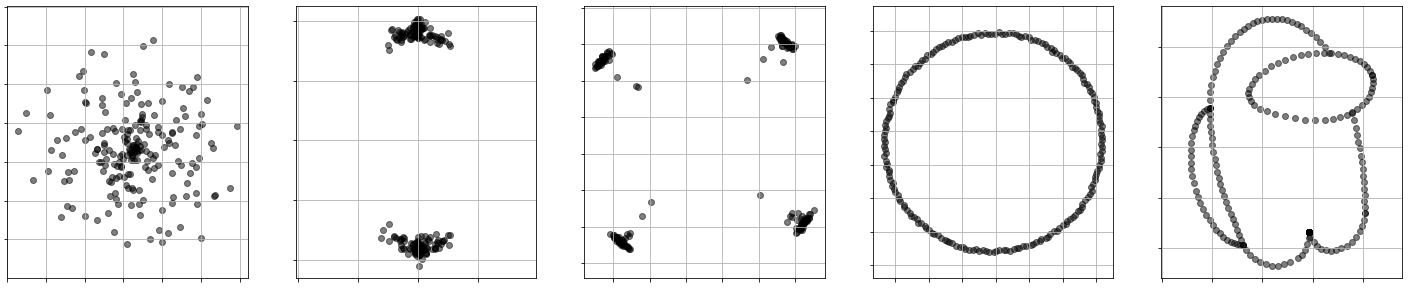
\includegraphics[width=1\linewidth]{./images/amongus.png}
    %Similar inputs with vastly different visualizations.}
    \caption{
    \small
    Various different 2D t-SNE visualizations produced by adversarial perturbations of a 200-point unit regular simplex. %\textcolor{red}{FIX THIS} high dimensional Gaussian.
    %Similar inputs with vastly different visualizations. 
    %The t-SNE visualization of five different 
    Each pair of perturbations satisfies the conditions of Theorem \ref{thm:perturbhammer} for $\epsilon = 0.01$.}
    \label{fig:sameIn_diffOut}
\end{figure}





\begin{lemma}\label{lem:image_of_tSNE}
    Fix any $n \geq 2$ and $\rho \in [1, n-1]$. For any $\epsilon>0$, define the set of $\epsilon$-perturbations of a unit simplex as $\Delta_\epsilon := \{ X=\{x_1, \dots, x_n\} \subset \mathbb{R}^{n-1}: \forall i\neq j, \lVert x_i - x_j \rVert^2 \in [1-\epsilon, 1+\epsilon]\}$. Then, for all $\epsilon>0$
    $${\IMTSNE} = {\TSNE}_\rho(\Delta_\epsilon).$$
\end{lemma}
%\todo[inline]{Corollary of this section is the perturbation result: As a consequence of this ``cluster exaggeration'', highly clustered visualizations can easily be perturbed by small changes in the input.}
%The key to understanding why this lemma holds is the \emph{additive invariance} property of t-SNE. 
In other words there is a set of datasets \(\Delta_\epsilon\) arbitrarily close to a regular unit simplex that generates \textit{all} possible stationary t-SNE outputs! This result indicates that t-SNE outputs are highly unstable on near-simplex inputs (cf.\ Figure \ref{fig:sameIn_diffOut}), which has real-world consequences since many high-dimensional datasets fall into this regime \citep{conc_hd_dist_1, aggarwal2001surprising} due to the concentration of measure phenomenon \citep{ledoux2001concentration}. %\textcolor{red}{We further investigate this instability through the lens of a single-point perturbations which we call \emph{poison point attacks}.}

\vspace{0.2in}
\subsubsection{Instability under insertion of a single point}

The previous lemma tells us that on intrinsically high-dimensional data, small perturbations of all the interpoint distances can have outsize effects on the t-SNE output. We observe that such datasets are susceptible to a much simpler adversarial attack: namely, the insertion of a \textit{single} data point. 

Consider a dataset $X$ sampled from a mixture of two high-dimensional Gaussians. t-SNE, as expected, reveals the two underlying clusters (see Figure \ref{fig:one_pt_perturb}, first panel). However, we can add just a single ``poison point" to $X$ and destroy the clustered visualization (see Figure \ref{fig:one_pt_perturb}, second panel; see also Figure \ref{fig:poison_point_scaling}). This failure mode of t-SNE is also observed on a real high-dimensional datasets (see Figures \ref{fig:outliers_real_world} and \ref{fig:bbc_appendix}, left vs.\ center). %Additional experiments are included the Appendix \ref{sec:appendix_outliers_experiment}.  %One striking feature of this single-point injection attack is that its efficacy persists even as the number of data points increases (see Figure \ref{fig:poison_point_scaling}).

How can a single point do so much damage? The answer lies in how t-SNE registers neighborhood information and its potential consequences in high dimensions. In the case of Figure \ref{fig:one_pt_perturb}, the poison point is placed at the mean of the dataset (this is captured clearly by the PCA plot). Due to the high dimensionality of the configuration (indeed, this mixture of two Gaussians is approximately a regular simplex) the poison point is the nearest neighbor to most of the points in the dataset. This significantly changes the input affinity matrix, downweighting the intra-cluster affinities and upweighting affinity for the poison point, resulting in a visualization which keeps points in tight proximity to their nearest neighbor (namely, the poison point). %It turns out that this severely disrupts the neighborhood information recorded in the input affinity matrix, 

This disproportionate amount of affinity towards the poison point is modulated by the perplexity value. As \(\rho\) decreases, the proportion of affinity placed on the poison point increases. In the limiting case, when \(\rho = 1\), \textit{all} affinity is assigned to the poison point. We can formalize this case as follows: 
%, completely obscuring the rest of the neighborhood information


%The mechanism behind the poison point attack can be understood in terms of how the input affinity matrix registers nearest neighbor information. When the poison point is placed such that it becomes the nearest neighbor of many other points, this can disrupt the more relevant nearest-neighbor information recorded in the input affinity matrix \(P\) and thus compromise the faithfulness of the embedding.  This effect is observed most drastically for low perplexity values. In the limiting case, when \(\rho = 1\), the \(P\) matrix becomes \textit{exactly} a symmetrized nearest-neighbors graph, and we can formalize the destructive impact of the poison point.


\begin{restatable}{theorem}{PoisonPoint} 
\label{thm:poison_point}
Take \(n\geq 4\) even. There exists two \(n\)-point datasets such that:
\begin{itemize}
    \item \(X_0 \subset \mathbb{R}^{n-1}\) has silhouette score \(0\) with respect to all partitions, and
    \item \(X_1\subset \mathbb{R}^{n-1}\) has silhouette score \(\frac{\sqrt{3}-1}{\sqrt{3}}\geq 0.42\) with respect to some partition of points,
\end{itemize}
yet there exists \(x_0\in \mathbb{R}^{n-1}\) such that (for \(\rho = 1\))
$$
{\TSNE}_\rho(X_0\cup x_0)={\TSNE}_\rho(X_1\cup x_0).
$$
  %  where \(I(A;B) = H(A) - H(A|B)\) denotes the mutual information between two random variables.
\end{restatable}

Therefore the poison point attack can make it \textit{impossible} to distinguish between a well-clustered and a completely un-clustered input based on their t-SNE loss landscapes (this is experimentally corroborated in Figure \ref{fig:poison_point_thm}). %\footnote{Note that it is easy to verify experimentally that t-SNE run on our constructions of the \(X_0\) and \(X_1\) yield the expected behavior: \(X_0\) registers as a blob, \(X_1\) as two well-separated clusters; see Appendix for experiments.} 
Our practical demonstrations (e.g.\ Figures \ref{fig:one_pt_perturb}, 
\ref{fig:outliers_real_world}, \ref{fig:poison_point_scaling},
\ref{fig:bbc_appendix}) indicate that a similar level of degradation persists for typical settings of \(\rho\) in the usage of t-SNE.


%and the intuition behind the proof suggest that a poison point attack---in the sense of simply injecting a point at the mean of the data or some subset thereof---can do significant damage in the regime whenever \(\rho\) is relatively small and the data is intrinsically high-dimensional (i.e.\ near regular simplex).


%One can imagine generalizations of Theorem \ref{thm:poison_point} which 



%We explore the poison point phenomenon further in the next section, where we contrast it with t-SNE's strikingly indifferent response to the injection of outlier points.



\begin{figure}
    \centering
       %
\includegraphics[width=\linewidth]{./images/poison_point/poison_point_3panel.png}  
       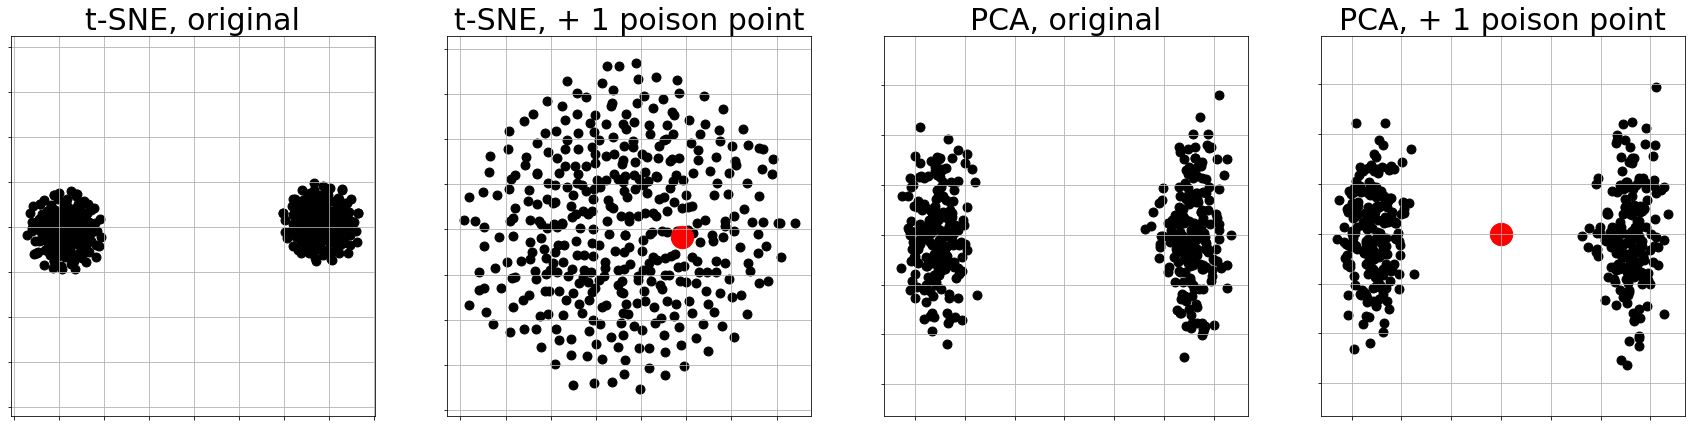
\includegraphics[width=\linewidth]{./images/outlier_figs/one_pt_perturb.png}
    %\vspace{-0.1in}
    \caption{    \small
     t-SNE versus PCA's radically different responses to the injection of a single ``poison'' point in the input dataset. The original dataset, visualized in panels 1 and 3, 
      consists of \(400\) points sampled from a mixture of two Gaussians in \(\mathbb{R}^{2000}\). The poison point is then placed at the mean of the previously sampled points; the resulting $401$ point dataset is visualized in panels 2 and 4. Note that this behavior persists for larger datasets, see Appendix \ref{sec:appendix_outliers_experiment}.}
      \label{fig:one_pt_perturb}
   % \vspace{-0.1in}
\end{figure}







%\todo[inline]{Add discussions of expansions of Theorem \ref{thm:unclustHammer} to other data visualization methods and cluster indices due to the widespread applicability of the proof technique.}

